\section{Meta-Heuristiken}
\subsection{Hill-Climbing \skript{2}}
  Konvergiert meist in lokales Optimum, Konvergenz sehr langsam., Wahl eines Zufallsschritts ist schwierig. Zielfunktion muss oft berechnet werden.
  
  Algorithmus, um Zielfunktion $f(\vec{x})$zu maximieren:
  \begin{enumerate}
    \item Start: Wahl von $\vec{x}^{alt}$
    \item Neue Wahl $\vec{x}^{neu}$ "`in der Nähe"' von $\vec{x}^{alt}$ (zuällig)%{\tiny (Das war die komische Bitschieberei in der Vorlesung)}
    \item Wenn $f(\vec{x}^{neu}) \geq f(\vec{x}^{alt})$, setze $\vec{x}^{alt} = \vec{x}^{neu}$ und gehe zu Schritt 2
  \end{enumerate}
  
 

\subsection{Tabu-Search \skript{3}}
  Grundidee: Keine / möglichst wenige Schritte, welche die Wirkung früherer Schritte rückgängig machen.
  
  Etwas schnellere Konvergenz ggn. Hill-Climbing, allerdings aufwendiges Mitführen und Aktualisieren der Tabu-Liste sowie Schwierigkeit, um Länge der Tabu-Liste zu finden. Zielfunktion muss oft berechnet werden.
  
  Algorithmus, um Zielfunktion $f(\vec{x})$zu maximieren:
  \begin{enumerate}
    \item Start: Wahl von $\vec{x}^{alt}$
    \item Neue Wahl $\vec{x}^{neu}$ "`in der Nähe"' von $\vec{x}^{alt}$, welche mit einem erlaubten Schritt $m_i \notin T$ eine möglichst gute Verbesserung (oder geringste Verschlechterung bringt).
    \item Einfügen des komplementären Schritts $\bar{m}_i$ in Tabu-Liste $T$.
    \item Schritte 2 und 3 wiederholen, bis vorgegebenes Abbruchkriterium erreicht ist.
  \end{enumerate}

\subsection{Simulated Annealing \skript{5}}
  Grundidee: Gegenüber dem Tabu-Search wird eine Verschlechterung der Lösung mit einer gewissen Wahrscheinlichkeit akzeptiert. So kann ein lokales Optimum wieder verlassen werden.
  
  \begin{enumerate}
    \item Start: Wahl von $\vec{x}^{alt}$
    \item Neue Wahl $\vec{x}^{neu}$ "`in der Nähe"' von $\vec{x}^{alt}$
    \item Wenn $f(\vec{x}^{neu}) \geq f(\vec{x}^{alt})$ oder mit einer Wahrscheinlichkeit von $p = e^{\frac{-\Delta E}{T}}$, setze $\vec{x}^{neu} = \vec{x}^{alt}$.\\
    Metropolis Regel: Zufallsvaribale $z \in [0,1]$. Wenn $z \leq p$ dann wird der schlechtere Wert genommen $\vec{x}^{neu} = \vec{x}^{alt}$
    \item Schritte 2 und 3 wiederholen, bis vorgegebenes Abbruchkriterium erreicht ist.
  \end{enumerate}
  
  Wahl der Parameter:
  \begin{itemize}
    \item $\Delta E$: Wenn Minimum: $\Delta E = f(\vec{x}^{neu}) - f(\vec{x}^{alt})$; wenn Maximum: $\Delta E = f(\vec{x}^{alt}) - f(\vec{x}^{neu})$
    \item Veränderung der Temperatur $T(i)$ (Kühlschema): Konstant, arithmetisch (bei jedem Schritt wird um gleichen Betrag verkleinert), geometrisch (bei jedem Schritt wird um gleichen Faktor verkleinert), stufenweise (diskrete Sprünge)
    \item Anfangstemperatur $T(0)$: Z.B. mittlere Änderung der Zielfunktion über einige zufällig gewählte Schritte.
  \end{itemize}
  

\subsection{Genetische Algorithmen (GA) \skript{8}}
  
    Löst alle Klassen von schwierigen Optimierungsproblemen: Parameteroptimierungen, kombinatorische Probleme (e.g. Travelling Salesman), Subset-Selektion (Stichwort Data-Mining). Nachteile sind die Erfahrung und das Geschick, das nötig ist für deren Entwicklung.
  
    Grundprinzip: Durch \em Selektion \em (Fitness/objective function), \em Rekombination \em (Kombination des genetischen Materials der Eltern) und \em Mutation \em (Veränderung der Erbinformation) können Funktionen optimiert werden. Dabei wird iterativ von einer "`alten"' Population durch verschiedene Operationen eine neue Population generiert, welche im Normalfall gleich gross sein soll.\\
    
  \begin{minipage}{12cm}  
    Beispiel eines GA-Modells:\\
    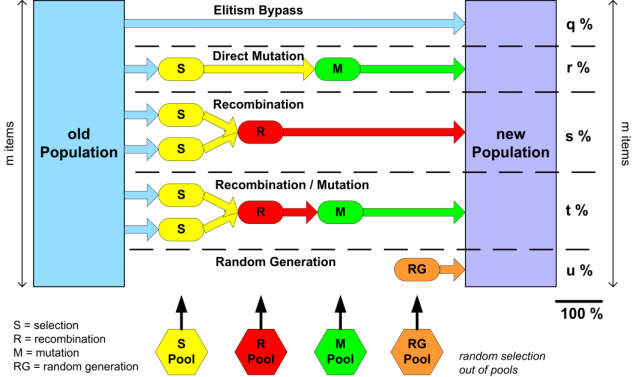
\includegraphics[width=12cm]{./Content/MetaHeuristics/GeneticAlgorithms_Model}
  \end{minipage}
  \begin{minipage}{6cm}
    \begin{flushright}
      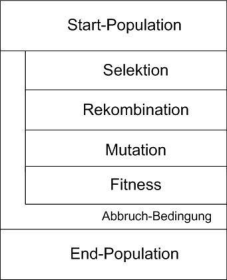
\includegraphics[width=5cm]{./Content/MetaHeuristics/GeneticAlgorithms_Principle}
    \end{flushright}
  \end{minipage}
  
  \begin{center}
    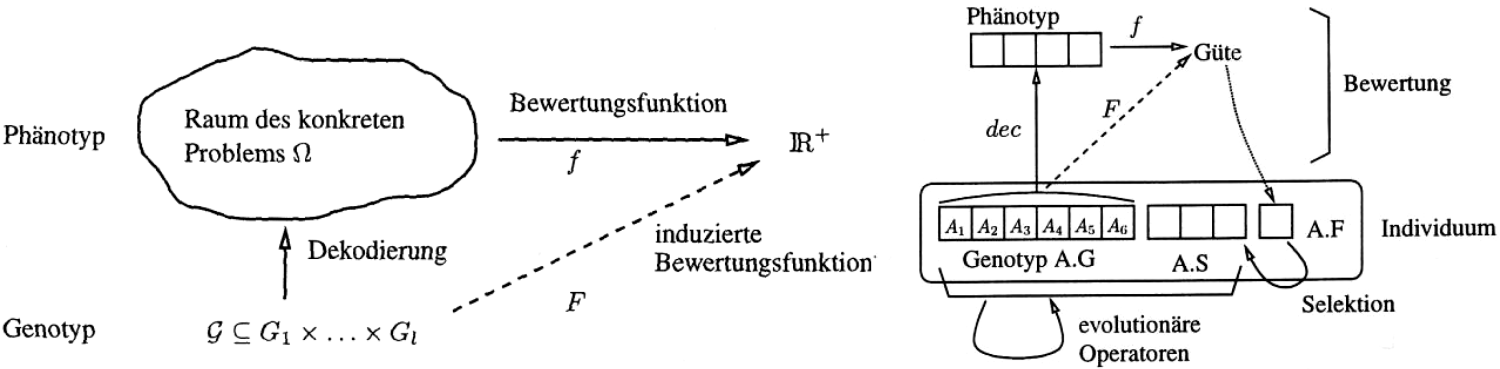
\includegraphics[width=0.7\textwidth]{./Content/MetaHeuristics/phenoGeno}
  \end{center}
  
    \subsubsection{Codierung der Parameter \skript{11}}
      Am besten werden die Parameter \em Gray\em -codiert. Damit wird erreicht, dass für jeden möglichen Parameter-Wert zwei Ein-Bit-Mutationen existieren, die den nächstgrösseren und -kleineren Parameter-Wert bilden.
      
      \begin{minipage}{0.33\textwidth}
      	\begin{center}
  	        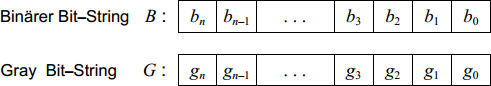
\includegraphics[width=\textwidth]{./Content/MetaHeuristics/GeneticAlgorithms_Gray}
  	      \end{center}
  	      $$g_j = \begin{cases}
  	        b_n                & j=n\\
  	        b_{j+1} \oplus b_j & j < n
  	        \end{cases} \qquad 
  	      b_j = \sum \limits_{k=n}^j \oplus g_k$$
      	\end{minipage}
      	\hfill
      	\begin{minipage}{0.3\textwidth}
            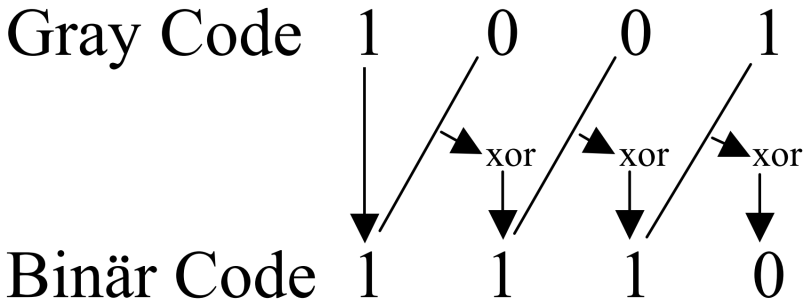
\includegraphics[width=\textwidth]{./Content/MetaHeuristics/binGray}	
    	\end{minipage}
    	\hfill
    	\begin{minipage}{0.3\textwidth}
            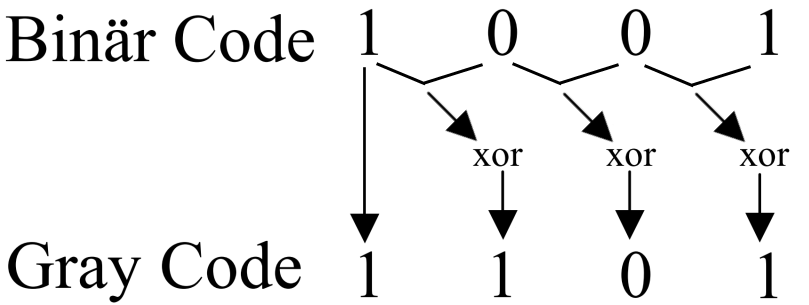
\includegraphics[width=\textwidth]{./Content/MetaHeuristics/grayBin}    	
    	\end{minipage}
  
  	Eine optimale Kodierung wurde dann vorliegen, wenn eine kleine Änderung am Genotypen eine kleine Änderung am Phänotyp bewirkt und wenn eine grosse Änderung am Genotypen auch eine grosse Änderung am Phänotyp zur Folge hat.

\subsubsection{Selektion \skript{15}}
  Probabilistische (Zufallsprinzip, z.B. \em Roulette-Wheel\em ) oder deterministische (nach Fitnesswerten, z.B. nur die besten; z.B. \em Binäre Wettkampfselektion\em ) Selektion. Problem bei beiden: Die besten Gene können verloren gehen, deshalb werden meist das beste oder die besten Individuen übernommen.
  
\subsubsection{Rekombination \skript{16}}
  \begin{tabularx}{\textwidth}{p{9cm} p{9cm}}
    \em One-Point Crossover\em : Der "`Chromosomen"'-String wird an zufälliger Stelle getrennt und neu rekombiniert: 
      & \em Two-Point Crossover\em : Der "`Chromosomen"'-String wird an zwei zufälligen Stellen getrennt und neu rekombiniert: \\
    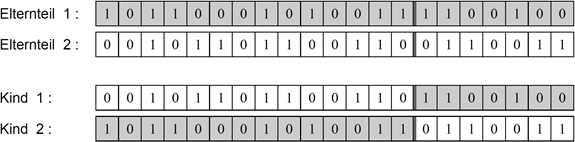
\includegraphics[width=8cm]{./Content/MetaHeuristics/GeneticAlgorithms_OnePointCrossover}
      & 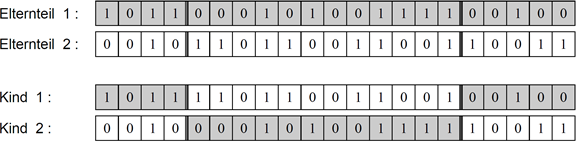
\includegraphics[width=8cm]{./Content/MetaHeuristics/GeneticAlgorithms_TwoPointCrossover} \\ \\
    \em $k$-Point Crossover\em : Verallgemeinerung von One-/Two-Point Crossover.
      & \em Uniform Crossover\em : $k$-Point Crossover mit Grenzwert $k \rightarrow n$, hier wird also jedes Bit zufällig kombiniert.
  \end{tabularx}
   
  
\subsubsection{Mutation \skript{18}}
  \begin{minipage}{7.75cm}
    \begin{itemize}
      \item \em Bit-Flip-Mutation\em : Zufällig ausgewählte Bits werden invertiert, wobei dies mit (kleiner) Wahrscheinlichkeit (Mutationsrate) geschieht.
      \item \em Positionsmutation\em : Bits oder ganze Bitstrings können an verschiedenen Positionen ausgetauscht werden.
      \item \em Inversion\em : Bits können auch invertiert werden (Auswahl durch Zufall).
    \end{itemize}
  \end{minipage}
  \hfill
  \begin{minipage}{10.75cm}
    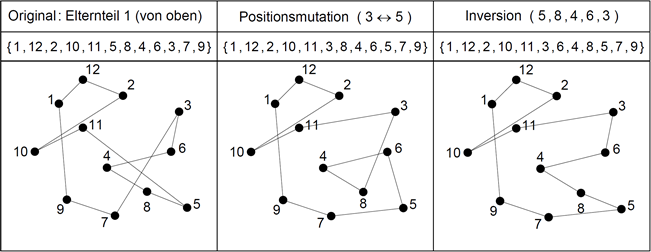
\includegraphics[width=11cm]{./Content/MetaHeuristics/GeneticAlgorithms_Mutation}
  \end{minipage}
  
  \newpage
  
\subsubsection{Ersetzungsschemata \skript{19}}

  Was passiert mit der alten Population?\\
  
  
  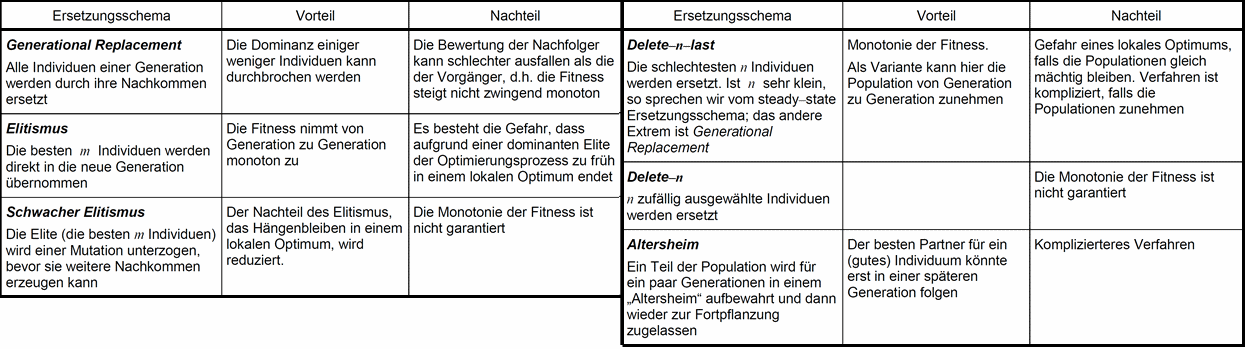
\includegraphics[width=\linewidth]{./Content/MetaHeuristics/GeneticAlgorithms_ReplacementsCroped}
   
   
  \subsection{Ant Colony Optimization \skript{21}}
  Ameisen folgen intensiven Pheromon-Spuren, da dort die Chance auf Futter zu treffen gross ist. Diese Idee wird bei ACO aufgenommen. Mit einer Wahrscheinlichkeit $P(x_{ij})$ wird ein möglicher Pfad $ij$ in die neue Generation übernommen. Zusätzlich wird meist auch ein "`Elite-Bypass"' mit Schwellwert $Q \in [0,1]$ implementiert:
  
  $$P(x_{ij}) = \begin{cases} \dfrac{\tau_{ij}^\alpha \eta_{ij}^\beta}{\sum\limits_{j \in \mathbf{W}_i} \tau_{ij}^\alpha \eta_{ij}^\beta}  & \text{if }j \in \mathbf{W}_i\\ 0 & \text{if }j \notin \mathbf{W}_i \end{cases}
  \qquad \qquad
  P(x_{ij}) = 
  \begin{cases}
    \text{if } z < Q = 
    \begin{cases}
      1 & \text{if } j = \arg \max\limits_{k \in \mathbf{W}_i}[\tau_{ik}^\alpha \eta_{ik}^\beta] \\
      0 & \text{else}
    \end{cases} \\
    \text{if } z \geq Q
    \begin{cases}
      \dfrac{\tau_{ij^\alpha \eta_{ij}^\beta}}{\sum\limits_{j \in \mathbf{W}_i} \tau_{ij}^\alpha \eta_{ij}^\beta}  & \text{if }j \in \mathbf{W}_i\\
      0 & \text{else}
    \end{cases}
  \end{cases}$$
  
  mit $\eta_{ij}$ als heuristischer Information (z.B. Abstand $\eta_{ij} = \frac{1}{d_{ij}}$ beim TSP), $z$ ist eine gleichverteilte Zufallsvariabale im bereich $[0,1]$.
  
  Bei jedem Schritt verdunsten die Pheromone nach folgender Regel mit Verdunstungsfaktor $0 \leq \rho \leq 1$:
  $$\tau_{ij}^{neu} = \begin{cases}
    \tau_{ij}^{alt} (1-\rho) + \frac{\rho}{f(\vec{x})} & \text{if } j \in \mathbf{W}_i\\
    \tau_{ij}^{alt} (1-\rho) & \text{if } j \notin \mathbf{W}_i\\
  \end{cases}
  \qquad \qquad
  \tau_{ij}^{neu} = \varphi \cdot \tau^0 + (1-\varphi) \cdot
  \begin{cases}
      \tau_{ij}^{alt} (1-\rho) + \frac{\rho}{f(\vec{x})} & \text{if } j \in \mathbf{W}_i\\
      \tau_{ij}^{alt} (1-\rho) & \text{if } j \notin \mathbf{W}_i\\
    \end{cases}
  $$
  
  ACO kann lokalen Extremalstellen konvergieren. Die kann durch das einführnen einer Konvergenzbremse $\varphi$ abgeschwächt werden.
  
  ACO wird eingesetzt für TSP, Vehicle Routing, Graph Coloring, Routing, Scheduling, etc.
  
  ACO liefert schnell gute Resultate für kombinatorische Probleme, ist aber nicht für Parameteroptimierung geeignet.\\
  
  \lstinputlisting[language=Java]{./Content/MetaHeuristics/ACO2.java}
  
\subsection{Particle Swarm Optimization \skript{23}}
  Speziell für Parameteroptimeriung geeignet: Jedes Individuum versucht zwar, sein lokales Optimum zu finden, gleichzeitig lernt es aber von den seinen eigenen Erfahrungen und denen des Schwarms.
  
  \begin{center}
  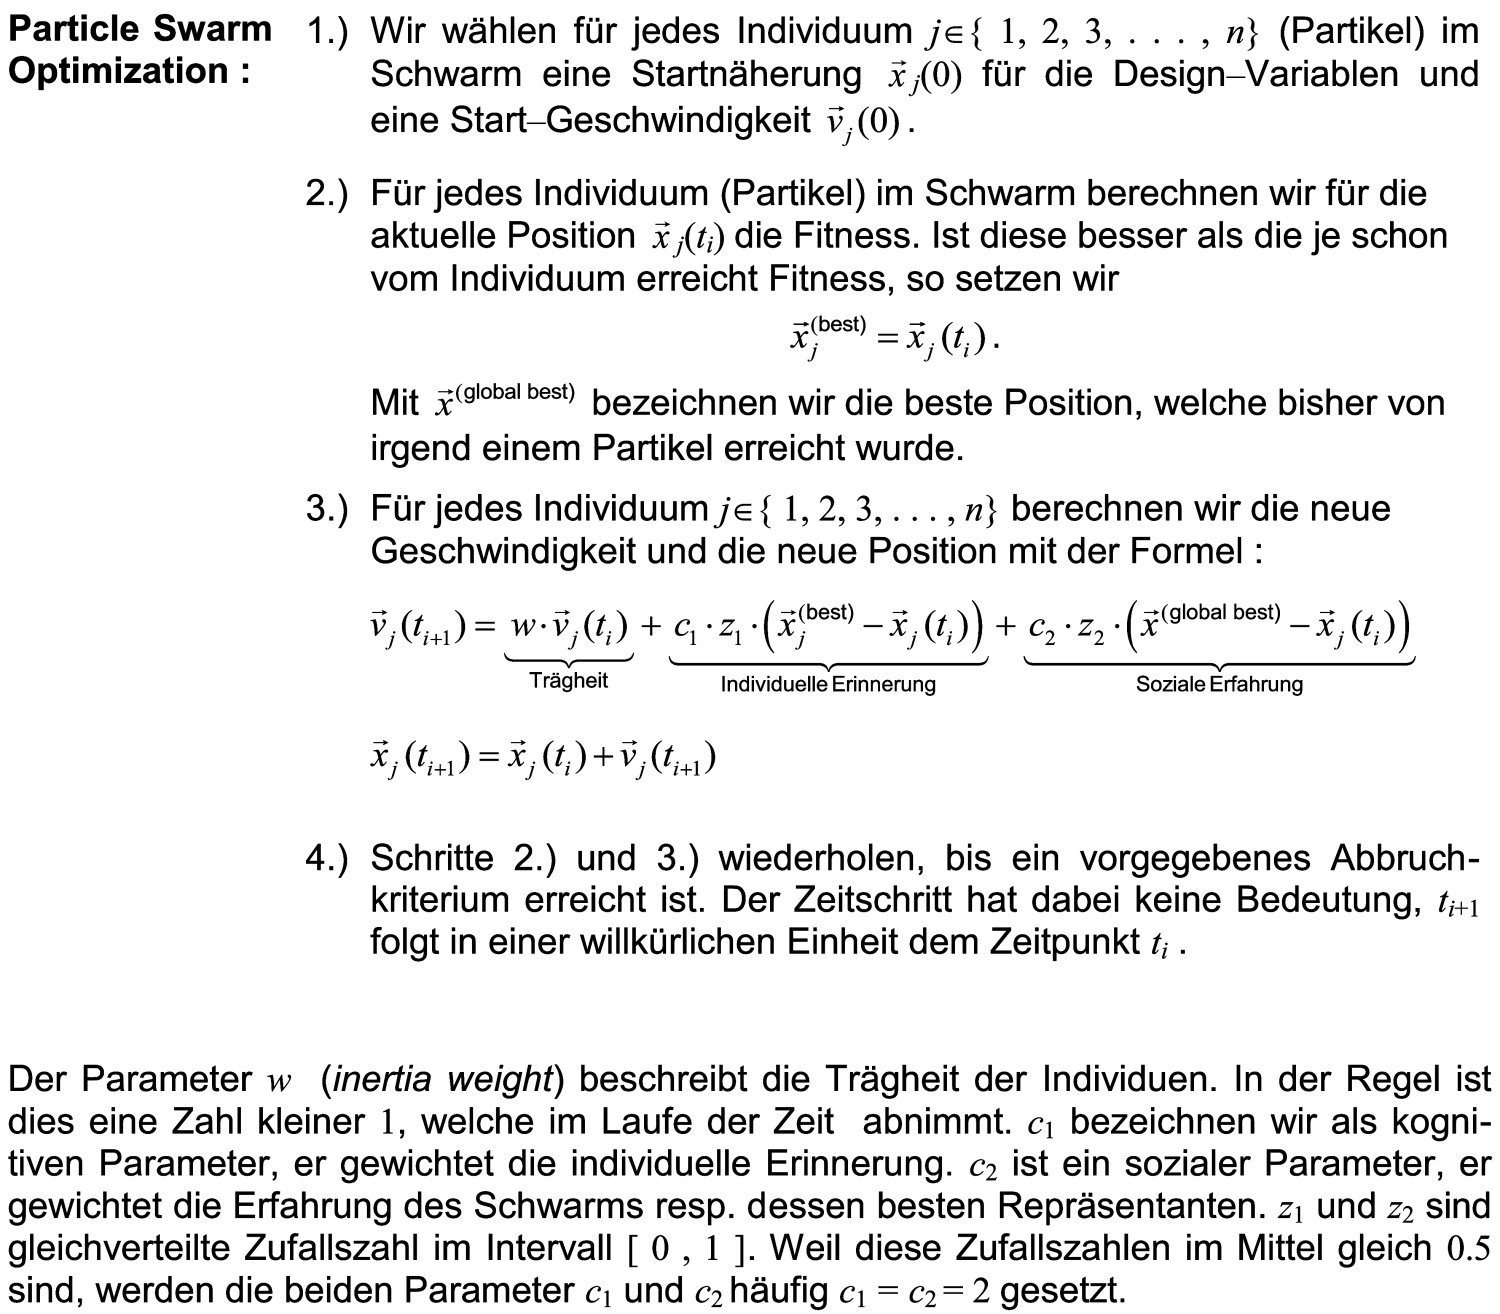
\includegraphics[width=0.7\linewidth]{./Content/MetaHeuristics/partSwarm}
  \end{center}

\newpage
  
  \lstinputlisting[language=Java]{./Content/MetaHeuristics/PSO2.java}
  

